\chapter{Marco teórico}
	
	\section{El agua}

	El planeta Tierra es conocido como planeta azul debido a que el \qty{70}{\percent} de su superficie está cubierta de agua, a pesar de ello, solamente el \qty{0.025}{\percent} de ella es potable. El \qty{97.5}{\percent} corresponde a al agua salada de mares y océanos; del \qty{2.5}{\percent} restante \qty{80}{\percent} está congelada en casquetes polares, glaciares o se encuentra como humedad del suelo y no se considera accesible. El resto se encuentra en el subsuelo, pozos, acuíferos, cuencas hidrográficas, ríos y arroyos \cite{el-dessouky_chapter_2002}.
	
	\subsection{Clasificaciones del agua}
	
		El agua puede clasificarse de distintas formas, entre las cuales se puede considerar el \acrfull{tsd}. En la~\cref{table:clasificacion-agua-tds} se puede observar la clasificación propuesta por la \acrfull{wqa}.
		
		\begin{longtblr}[
			caption = {Clasificación del agua con respecto al \acrshort{tsd} según \acrshort{wqa}},
			label = {table:clasificacion-agua-tds},
			remark{Referencia} = {Datos obtenidos del glosario en línea de la \acrshort{wqa} \cite{water_quality_association_glossary_nodate}}
		]{
			colspec = {*{2}{X[c]}},
			width=0.7\textwidth,
			hlines,
			vlines,
			row{odd} = {bg=tablerowblue},
			row{1} = {
				bg = tabletitleblue,
				fg=white,
				font =  \large\bfseries
			},
			rowhead = 1,
			rows={m},
		}
			{Denominación} & TSD (\unit[per-mode = symbol]{\mg\per\litre})\\ 
			% Table body%
			Agua fresca & menor a \num{1000}\\
			Agua salobre & entre \num{1000} y \num{5000}\\
			Agua altamente salobre & entre \num{5000} y \num{15000}\\
			Agua salina & entre \num{15000} y \num{30000}\\
			Agua de mar & entre \num{30000} y \num{40000}\\
			Salmuera & entre \num{40000} y \num{300000}+\\
		\end{longtblr}
		
		Otra forma de clasificar el agua es de acuerdo a su forma final de uso y la salinidad que presenta. En la~\cref{table:clasificacion-agua-dessouky} se describe la relación entre el grado de salinidad y su uso en sectores de la población.
		
		\begin{talltblr}[
			caption = {Clasificación del agua propuesta por \cite{el-dessouky_chapter_2002} de acuerdo a su uso},
			label = {table:clasificacion-agua-dessouky}
		]{
			colspec = {X[c] X[0.75, c] X[c]},
			width=\textwidth,
			hlines,
			vlines,
			row{odd} = {bg=tablerowblue},
			row{1} = {
				bg = tabletitleblue,
				fg=white,
				font =  \large\bfseries
			},
			rowhead = 1,
			rows={m},
			cell{3}{3} = {r=2}{valign = m}
		}
			{Categoría} & Salinidad (ppm) & Fuentes\\ 
			% Table body%
			Industrias como la farmacéutica, eléctrica o de evaporación en calderas
				& menor a \num{5}
				& Ríos de muy baja salinidad o plantas desalinizadoras\\
			Agua potable
				& menor a \num{150}
				& Ríos, Lagos, plantas desalinizadoras\\
			Agua para uso doméstrico 
				& entre \num{150} y \num{1000}
				&~\\
			Riego y refrigeración industrial
				& entre \num{1000} y \num{3000}
				& Agua salobre y agua de mar\\		
		\end{talltblr}
	
	\subsection{Composición del agua de mar}
	
		El agua de mar es una mezcla compleja de aproximadamente \percent{96.5} de agua y \percent{2.5} de sales y en menor cantidad otras sustancias incluyendo sustancias orgánicas e inorgánicas disueltas \cite{alyn_c_duxbury_seawater_2023}.
		
		\subsubsection{Propiedades químicas y físicas del agua de mar}
		
			El agua de mar contiene seis iones predominantes los cuales pueden ser observados en la~\cref{table:ionic-composition-of-seawater} junto a otros iones en menor cantidad.
			
			La composición química del agua en mar abierto es constante aunque los \acrshort{tsd} varían de acuerdo a las condiciones locales; esto se puede atribuir a la diferencia de tiempo que existe entre la difusión y el tiempo de abastecimiento del agua.
			
			\begin{longtblr}[
				caption = {Principales iones constituyentes del agua de mar},
				label = {table:ionic-composition-of-seawater},
				remark{Nota} = {Concentración de salinidad igual a \num{34.7}},
				remark{Referencia} = {Tabla traducida de \cite{alyn_c_duxbury_seawater_2023}}
			]{
				colspec = {*{4}{X[c]}},
				width=\textwidth,
				hlines,
				vlines,
				row{odd} = {bg=tablerowblue},
				row{1} = {
					bg = tabletitleblue,
					fg=white,
					font =  \large\bfseries
				},
				rowhead = 1,
				rows={m}
			}
				Constituyente iónico
					& Compuesto químico
					& \unit{\gram\per\kg\ de\ agua}
					& \unit{\mole\per\kg\ de\ agua}\\
				Cloruro
					& \ch{Cl\mch}
					& 19.162
					& 0.5405\\
				Sodio
					& \ch{Na\pch}
					& 10.679
					& 0.4645\\
				Magnesio
					& \ch{Mg\pch[2]}
					& 1.278
					& 0.0526\\
				Sulfato
					& \ch{(SO4)\mch[2]}
					& 2.680
					& 0.0279\\
				Calcio
					& \ch{Ca\pch[2]}
					& 0.4096
					& 0.01022\\
				Potasio
					& \ch{K\pch}
					& 0.3956
					& 0.01011\\
				Ácido carbónico
					& \ch{(CO3)\mch[2]}
					& 0.0276
					& 0.0023\\
				Bromuro
					& \ch{Br\mch}
					& 0.0663
					& 0.00083\\
				Boro
					& \ch{B}
					& 0.0044
					& 0.00041\\
				Estroncio
					& \ch{Sr\pch[2]}
					& 0.0079
					& 0.00009\\
				Fluoruro
					& \ch{F\mch}
					& 0.0013
					& 0.00007
			\end{longtblr}
	
	\subsection{El efecto de la salinidad sobre el agua}
			
		Obianyo \cite{obianyo_effect_2019} realizó un experimento con diferentes sales y cantidades para observar cómo afecta la salinidad la capacidad de evaporación del agua; su estudio nos indica que hay una relación clara entre el aumento de la salinidad y la reducción de la evaporación. Los coeficientes de retardo se pueden observar en la~\cref{table:retardo-evaporacion-sal}.
		
		En el \cref{ch:seawater-properties} podemos observar las propiedades del agua de mar a una atmósfera de presión \cites{nayar_thermophysical_2016}{sharqawy_thermophysical_2010}, en el que se puede corroborar la relación de la salinidad y diversas propiedades vinculadas a la evaporación.
		
		\begin{minipage}[c]{0.5\linewidth}
			\begin{talltblr}[
				caption = {Factores de retardo en la evaporación de agua con diferentes sales},
				label = {table:retardo-evaporacion-sal}
			]{
				colspec = {c c},
				hlines,
				vlines,
				row{odd} = {bg=tablerowblue},
				row{1} = {
					bg = tabletitleblue,
					fg=white,
					font =  \large\bfseries
				},
				rowhead = 1,
				rows={m},
			}
				
				{Sal} & Factor de retraso\\ 
				% Table body%
				Sulfato de magnesio & \num{0.800}\\
				Hidróxido de sodio & \num{0.490}\\
				Cloruro de sodio & \num{0.712}\\
				Cloruro de amonio & \num{0.820}\\
				Nitrato de potasio & \num{0.822}\\
			\end{talltblr}
		\end{minipage}
		\hfill
		\begin{minipage}[c]{0.45\linewidth}
			\begin{figure}[H]
				\centering
				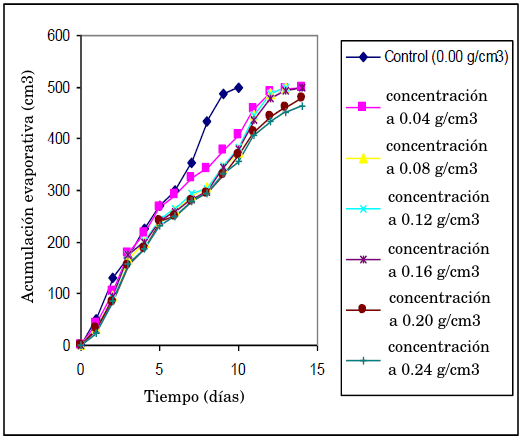
\includegraphics[width=\linewidth, keepaspectratio]{Marco-teórico/nacl-evaporation.png}
				\caption{Relación entre la evaporación acumulada y el tiempo para la solución NaCl}
				\floatfoot{Figura traducida de \cite{obianyo_effect_2019}}
				\label{fig:relacion-evaporación-sal}
			\end{figure}
		\end{minipage}
	\subsection{Propiedades coligativas del agua}
			
		El agua es un solvente por excelencia, por ello, en un proceso de desalinización se deben tomar en cuenta \gls{propiedades_coligativas} de las soluciones:
		
		\begin{itemize}[columns=2]
			\item Reducción relativa de la presión de vapor
			\item Elevación del punto de ebullición
			\item Depresión en el punto de congelación
			\item Presión osmótica
		\end{itemize}
		
		\subsubsection{Elevación del punto de ebullición y disminución de la presión de vapor}
			
			La elevación del punto de ebullición es proporcional a la molaridad de la solución. Este fenómeno se puede explicar a través de la presión de vapor.
			
			\begin{displayquote}
				La presión de vapor del líquido puro refleja la tendencia de la solución hacia una mayor entropía, que se puede lograr si el líquido se vaporiza para formar un gas. Cuando un soluto está presente, hay una contribución adicional a la entropía del líquido, incluso en una solución ideal. Debido a que la entropía del líquido ya es más alta que la del líquido puro, hay una tendencia más débil a formar el gas (\cref{fig:coligativas-pv}). El efecto del soluto aparece como una presión de vapor baja, y por lo tanto un punto de ebullición más alto. Del mismo modo, la aleatoriedad molecular mejorada de la solución se opone a la tendencia a congelarse. En consecuencia, se debe mantener una temperatura más baja antes de alcanzar el equilibrio entre el sólido y la solución. Por lo tanto, el punto de congelación se reduce. \cite{atkins_physical_2010}.
			\end{displayquote}
			\begin{figure}[H]
				\centering
				\begin{subfigure}[t]{0.45\linewidth}
					\centering
					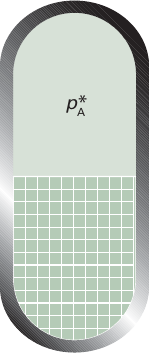
\includegraphics[width=\linewidth, height=50mm, keepaspectratio]{
						Marco-teórico/atkins-a.png
					}
					\caption{Se imagina a un solvente líquido como una estructura de cuadros}
				\end{subfigure}
				\hfill
				\begin{subfigure}[t]{0.45\linewidth}
					\centering
					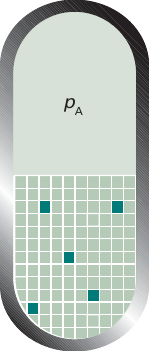
\includegraphics[width=\linewidth, height=50mm, keepaspectratio]{
						Marco-teórico/atkins-b.png
					}
					\caption{Cuando hay presencia de un soluto (cuadros oscuros), la entalpía es más grande a comparación de un líquido puro y por ello hay una decreciente tendencia a adquirir el desorden característico de un vapor}
				\end{subfigure}
				
				\caption{La presión de vapor de un líquido puro representa el balance entre el aumento de entalpía debido a la vaporización y la disminución de entalpía en su entorno.}
				\floatfoot{Figuras obtenidas de \cite{atkins_physical_2010}}
				\label{fig:coligativas-pv}
			\end{figure}
	\input{Content/Chapter-5/sections/Radiación-solar.tex}
	\input{Content/Chapter-5/sections/Concentración-solar.tex}
	\input{Content/Chapter-5/sections/Desalinización.tex}
%	\section{Termodinámica de la destilación solar}
	
	\subsection{Evaporación del agua}

		La evaporación es el fenómeno que ocurre en la interfase líquido-vapor cuando la presión de vapor es menor que la presión de saturación de un líquido a una temperatura dada. A diferencia de la ebullición, la evaporación puede suceder a cualquier temperatura, adquiriendo mayor rapidez entre más alta es la temperatura. \cite{cengel_transferencia_2010}

		La presión atmosférica es la suma de la presión del aire seco y la presión de vapor~\eqref{equ:presion-atmosferica}, esta última constituye generalmente menos de un \qty{3}{\percent} de la presión atmosférica.

		\begin{equation}\label{equ:presion-atmosferica}
			\gls{patm} = \gls{paire} + \gls{pvapor}
		\end{equation}

		El aire presenta límites de humedad pues es limitada la cantidad de vapor de agua que puede contener; podemos entonces definir a la humedad relativa \gls{humedad-relativa} como la relación de cantidad de vapor de agua real en el aire a determinada temperatura y la máxima cantidad que el aire puede contener a la misma temperatura. Para el aire seco $\gls{humedad-relativa} = 0$ y para el aire saturado $\gls{humedad-relativa} = 1$.

		Podemos entonces especificar por completo la cantidad de humedad en el aire si conocemos la temperatura y la humedad relativa; a su vez podemos relacionar la presión de vapor con la humedad relativa mediante la~\cref{equ:relacion-pv-psat}. Podemos notar que la presión de saturación incrementa conforme más humedad exista en el aire. \cite{cengel_termodinamica_2009}

		\begin{equation}\label{equ:relacion-pv-psat}
			\gls{pvapor} = \gls{humedad-relativa} P_{\text{sat a T}}
		\end{equation}
		
	\section{Ebullición del agua}

		La ebullición del agua es un proceso complejo de analizar pues comprende varias etapas, tanto si es ebullición en estanque como en flujo. La creación aparentemente aleatoria de burbujas y de películas de vapor hacen que no se pueda obtener de manera precisa un modelo matemático que describa el comportamiento de este fenómeno.

		\subsection{Ebullición en estanque}

			La ebullición en estanque presenta 4 regímenes de ebullición: ebullición en convección natural, ebullición nucleada, ebullición de transición y ebullición en película

			\begin{figure}[ht]
				\centering
				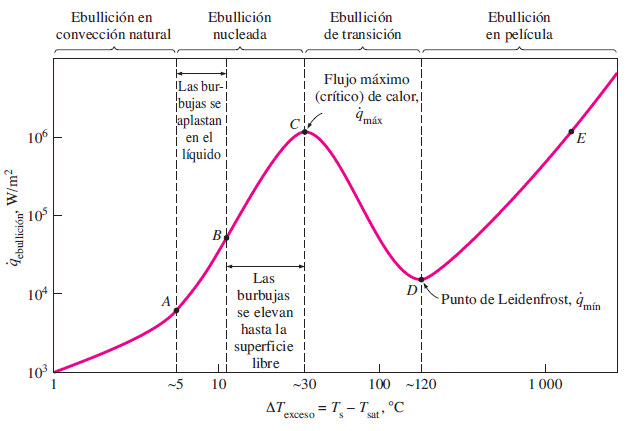
\includegraphics[width=\linewidth,height=90mm, keepaspectratio]{Marco-teórico/Regímenes-ebullición-en-estanque.png}
				\caption{Curva típica de ebullición en estanque del agua a 1 atmósfera}
				\floatfoot{Imagen obtenida de \cite{cengel_transferencia_2010}}
				\label{fig:regimenes-ebullicion-en-estanque}
			\end{figure}

			En la curva mostrada en la~\cref{fig:indice-estres-evaporativo} se puede apreciar no sigue un comportamiento lineal y el que la superficie tenga más temperatura no significa que aumentará la transferencia de calor, pues la formación de burbujas al cambiar de fase el agua disminuye esta razón y entre mayor sea esta capa de vapor, menor transferencia tendremos dada la menor conductividad térmica del vapor. En general, los procesos de ebullición no seguirán más allá de nuestro punto C, pues para lograr obtener otra vez la misma transferencia de calor se tendría que alcanzar el punto E, el cual alcanza temperaturas mayores al punto de fusión de varios de los materiales que usualmente son empleados durante estos procesos. Cabe mencionar que una vez alcanzado el punto de Leidenfrost, se observa que la transferencia de calor por radiación empieza a apreciarse y cuando la temperatura en exceso es demasiado alta, este mecanismo de transferencia se vuelve predominante.

		\subsection{Ebullición en flujo interno}

			La ebullición en flujo fuerza a un fluido a moverse por medio de una fuerza externa, este se considera en flujo interno si la superficie por la que fluye evita que el vapor escape, es decir un flujo dentro de un tubo. Este método de transferencia al ser bifásico es más complejo de analizar y se pueden distinguir 7 etapas visibles en la~\cref{fig:Regimenes-ebullicion-en-flujo-interno}. Es a su vez importante recordar que durante este fenómeno se presenta la condición de no deslizamiento.

			\begin{figure}[H]
				\centering
				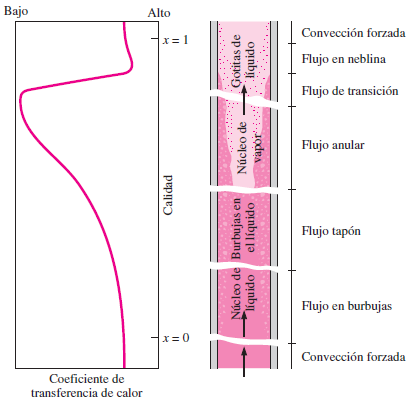
\includegraphics[width=\linewidth,height=90mm, keepaspectratio]{Marco-teórico/Regímenes-ebullición-en-flujo-interno.png}
				\caption{Curva típica de ebullición en estanque del agua a 1 atmósfera}
				\floatfoot{Imagen obtenida de \cite{cengel_transferencia_2010}}
				\label{fig:Regimenes-ebullicion-en-flujo-interno}
			\end{figure}

			\subsubsection{Convección interna forzada}

				{\textit{Geometría}}

				Como menciona \cite{cengel_transferencia_2010}, para un área superficial fija, el tubo circular da la mayor transferencia de calor para la caída de presión más baja, siendo popular su uso en el transporte de fluidos, en especial los líquidos, debido a que pueden soportar grandes diferencias de presión entre el ambiente y el volumen interno\footnote{Dado a lo aquí descrito, los puntos subsecuentes serán delimitados a los tubos circulares.}. Los tubos no circulares suelen usarse en sistemas de calefacción y enfriamiento.

				{\textit{Flujo}}

				El flujo de un sistema puede ser unidimensional, bidimensional o tridimensional de acuerdo a las variaciones a lo largo de las coordenadas donde podemos definir un vector $\vec{V}(x,y,z)$ o bien $\vec{V}(r,\theta,z)$ dependiendo del sistema de referencia que nos convenga analizar.

				En la entrada de un tubo circular se podría decir que tenemos un flujo bidimensional, pues las variaciones en la tercera coordenada serían demasiado pequeñas como para suponer una influencia en los cálculos, este flujo el entrar empieza a ganar uniformidad y después de cierta distancia (alrededor de 10 diámetros del tubo para flujo turbulento \cite{cengel_transferencia_2010}) se puede decir que el flujo está completamente desarrollado y para un tubo circular el flujo es unidimensional en este punto en coordenadas cilíndricas o bidimensional en coordenadas cartesianas.

				A su vez podemos distinguir entre un flujo laminar, turbulento o en transición. El flujo laminar se caracteriza por ser un movimiento altamente ordenado y con líneas suaves de corriente; por el contrario el flujo turbulento tiene fluctuaciones en la velocidad y presenta un movimiento altamente desordenado, por lo que la transferencia de calor es mucho mayor que en el flujo laminar, pues provee mayor interacción entre la materia. El cambio entre estos dos flujos al no ser repentino tiene una etapa de transición donde varía entre flujo laminar y turbulento.

				Este modelo de flujo depende de varios factores como la configuración geométrica de la superficie, las asperezas del material, la velocidad de flujo, la temperatura y las propiedades del fluido. En 1880, Reynolds descubrió que el régimen de flujo depende principalmente de la razón entre las fuerzas de inercia a las fuerzas viscosas. De ahí surge el número de Reynolds, el cual es una cantidad adimensional y se expresa como en la~\cref{equ:reynolds-number}

				\begin{equation}
					\label{equ:reynolds-number}
					\gls{reynolds} = \dfrac{V\gls{lc}}{v} = \dfrac{\gls{density} V\gls{lc}}{\mu}
				\end{equation}

				Donde:
				\begin{conditions}
					V & Velocidad corriente superior \\
					v & Viscosidad cinemática del fluido \\
					\mu & Viscosidad dinámica \\
					\rho & Densidad
				\end{conditions}

				{\textit{Velocidad y temperatura promedios}}

				Recordemos que por la condición de no deslizamiento, vamos a tener diferentes velocidades en el tubo, siendo cero en la superficie y alcanzando un máximo en el centro; por lo que el considerar una velocidad promedio se hace especialmente útil, obedeciendo al principio de la conservación de la masa.

				\begin{equation}
					\label{equ:average-velocity-internal-flow}
					V_{\text{prom}} = \dfrac{2}{R^2} \int_{0}^{R} u(r)rdr
				\end{equation}

				Donde:
				\begin{conditions}
					u(r) & Perfil de velocidad \\
					R & Radio
				\end{conditions}

				Algo similar ocurre con la temperatura, sin embargo, a diferencia de la velocidad promedio, la temperatura promedio varía conforme el fluido de desplaza. Esta temperatura obedece al principio de la conservación de la energía.

				\begin{equation}
					\label{equ:average-temperature-internal-flow}
					T_{\text{prom}} = \dfrac{2}{V_{prom}R^2} \int_{0}^{R} T(r)u(r)rdr
				\end{equation}

				Donde:
				\begin{conditions}
					u(r) & Perfil de velocidad \\
					R & Radio
				\end{conditions}
				
				
				{\textit{Análisis térmico}}

				El desplazamiento del fluido supone un ligero aumento de calor por la fricción entre las partículas, sin embargo, este aumento es tan pequeño que en realidad no afecta el cálculo general, por lo cual este cálculo se descarta, con excepción de líquidos intensivamente viscosos con altos gradientes de velocidad

				{\textit{Caída de presión}}

				La caída de presión es una cantidad que está relacionada de manera directa con la potencia requerida por las bombas o ventiladores para mantener un flujo dado \cite{cengel_transferencia_2010}. ``En la práctica, resulta conveniente expresar la pérdida de presión para todos los tipos de flujos internos completamente desarrollados (flujos laminares o turbulentos, tubos circulares o no circulares, superficies lisas o ásperas, tubos horizontales o inclinados) como"

				\begin{equation}
					\label{equ:caida-presion}
					\Delta P_{L} = f\dfrac{L}{D}\dfrac{\rho V_{promedio}^{2}}{2}
				\end{equation}

				Donde $f$ se conoce como el factor de fricción de Darcy o Darcy-Weisbach

				\begin{equation}
					\label{equ:ff-darcy}
					f = \dfrac{8\tau_{w}}{\rho V_{promedio}^{2}}
				\end{equation}

			\subsection{Intensificación de la transferencia de calor}

				Cengel \cite{cengel_transferencia_2010} nos indica que una manera de mejorar la transferencia de calor hacer intencionalmente que la superficie tenga asperezas o porosidades para favorecer la nucleación, por lo que a menudo las superficies de los tubos son ásperas, corrugadas o con aletas, teniendo importantes incrementos en la transferencia de calor con hasta un \qty{400}{\percent} de mejora, aunque este aumento viene acompañado de un incremento en el factor de fricción y caída de presión, otras maneras de mejorar esta transferencia son generadores de pulsos, al inducir remolinos.

				Ramírez \cite{ramirez_intensificacion_2018} realizó un trabajo donde aglomera distintos métodos para mejorar la razón de transferencia de calor en ebullición convectiva durante el flujo interno de un fluido revisando numerosos mecanismos entre los que se encuentran:

				\textit{Tubos con aletas internas}

				Las aletas internas son utilizadas para mejorar la transferencia de calor en flujos multifásicos y monofásicos; disminuyen el diámetro hidráulico a la vez que aumentan la superficie de contacto y aunque no presenta ínfimas ventajas para la nucleación tiene un considerable aumento en la convección de fluidos multifásicos.

				\begin{figure}[ht]
					\centering
					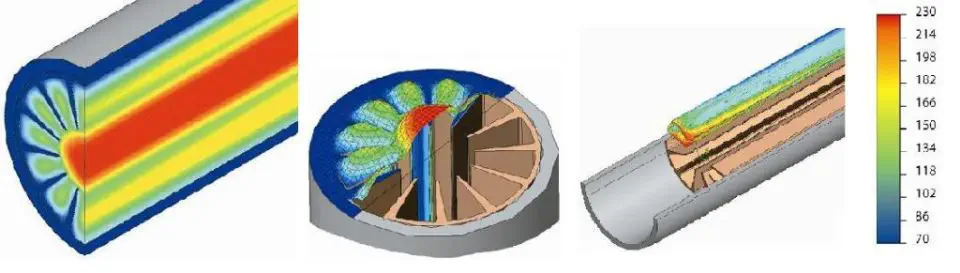
\includegraphics[width=\linewidth,height=50mm, keepaspectratio]{Marco-teórico/tubos-aletados.png}
					\caption{Tubo con aletas internas}
					\floatfoot{Imagen obtenida de \cite{direct_industry_tubos_nodate}}
					\label{fig:tubos-aletados}
				\end{figure}

				\textit{Tubos microaletados}

				Aunque son tubos usualmente utilizados para la refrigeración y aire acondicionado \cites{wang_single-phase_1996}{greco_convective_2008} citados por \cite{ramirez_intensificacion_2018} pudieron mostrar que los incrementos en tubos con microaletas tienen incrementos en el intercambio de calor de $1.6$ a $3.2$ veces, siendo las causas principales:

				\begin{itemize}[columns = 2]
					\item Aumento del área de contacto
					\item El área de levantamiento en la dirección de la circunferencia es grande
					\item Aumento de cavidades para la nucleación
					\item Las aletas tienen un efecto sobre la tubulencia y el flujo secundario
				\end{itemize}

				\begin{figure}[htb]
					\centering
					 \begin{subfigure}[H]{0.6\textwidth}
				         \centering
				         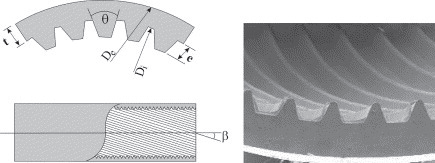
\includegraphics[width=\linewidth,height=50mm, keepaspectratio]{Marco-teórico/tubo-microaletado.png}
				         \caption{Geometría del tubo}
				         \label{fig:tubo-microaletado}
				     \end{subfigure}
				     \hfill
				     \begin{subfigure}[H]{0.3\textwidth}
				         \centering
				         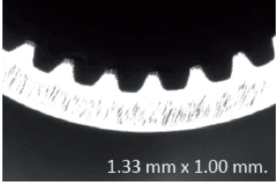
\includegraphics[width=\linewidth,height=50mm, keepaspectratio]{Marco-teórico/tubo-microaletado-cerca.png}
				         \caption{Perfil de la aleta }
				         \label{fig:tubo-microaletado-cerca}
				     \end{subfigure}
					\caption{Tubos con microaletas}
					\floatfoot{Imagen obtenida de \cite{ramirez_intensificacion_2018}}
					\label{fig:tubos-microaletados}
				\end{figure}

				\textit{Arreglo de tubos de cintas torcidas}

				Este arreglo es ampliamente usado para flujos monofásicos, sin embargo, también son dispositivos muy eficaces en el aumento de la razón de transferencia de calor, dado a que estos arreglos centrifugan el líquido contra la pared desplazando el vapor y reduciendo el diámetro hidráulico, también propician remolinos que incrementan la interacción de la materia y energía aunque también \textbf{existe una caída de presión importante}.

				\begin{figure}[ht]
					\centering
					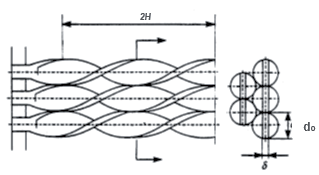
\includegraphics[width=\linewidth,height=50mm, keepaspectratio]{Marco-teórico/arreglo-cintas-torcidas.png}
					\caption{Arreglo de cintas torcidas}
					\floatfoot{Imagen obtenida de \cite{ramirez_intensificacion_2018}}
					\label{fig:cintas-torcidas}
				\end{figure}

				\textit{Campos acústicos}

				En el estudio de Ramírez se menciona que hay diversos estudios que han demostrado que los efectos acústicos en las burbujas cercanas a la pared calentada tienen una influencia importante en la transferencia de calor apresurando el desprendimiento de las burbujas que se adhieren a las paredes del tubo.
	
%	\subsection{Aumento de temperatura}
%		
%		La energía térmica o calor así mismo como el sonido, es el movimiento vibracional de los átomos y moléculas. Las vibraciones de baja frecuencia corresponden al sonido mientras que frecuencias más altas se expresan en forma de calor \cite{chandler_explained_2010}. A la energía asociada a esta excitación se le conoce como fonón.
%		
%		La cantidad de energía térmica en un cuerpo definirá la temperatura de este y su incremento se puede cuantificar a través de~\eqref{equ:incremento-temperatura}
%		
%		\begin{equation}
%			\label{equ:incremento-temperatura}
%			\Delta\gls{T} = \dfrac{\gls{Q}}{\gls{cs}\gls{m}}
%		\end{equation}
%	
%	\subsection{Pérdidas de calor}
%		
%		\subsubsection{Convección}
%			dsfdsf
		
%		A diferencia de los fotones, los fonones interactúan entre sí incluso si tienen diferentes longitudes de onda, por lo que su interacción se vuelve más caótica
	
	
			
			%Los recubrimientos protectores son particularmente eficaces para controlar la corrosión uniforme. La protección catódica (CP), una técnica electroquímica utilizada para el control de la corrosión, se puede utilizar en situaciones subterráneas o de inmersión.
				
			
			
			%rodriguez_suarez_industria_2017 
		
		%garcia_garrido_guitecnica_2012 pp30